%%This is a very basic article template.
%%There is just one section and two subsections.
\documentclass[parskip=full]{scrartcl}
\usepackage[table]{xcolor}

\usepackage{amsmath}
\usepackage{amsfonts}
\usepackage{mathtools}
\usepackage{studarbeit}
\usepackage{graphicx}
\usepackage{wrapfig}
\usepackage{lscape}
\usepackage{rotating}
\usepackage{epstopdf}
\usepackage{pdfpages}
\usepackage{caption, booktabs}
\usepackage{tabularx}
\usepackage{multirow}
\usepackage{here}
\usepackage[most]{tcolorbox}
\usepackage[binary-units=true]{siunitx}
 \usepackage[autostyle=true,german=quotes]{csquotes}
 \usepackage{longtable, booktabs}
 \newcommand{\swtLabel}[1]{\textbf{/#1\arabic*0/}}
 \renewcommand{\labelitemii}{~}
 %\renewcommand{\labelitemi}{~}
 \newcommand{\fehler}[4]{\textbf{#1}
 							\begin{itemize}
 							  \item \textbf{Symptom}  #2
 							  \item \textbf{Grund} #3
 							  \item \textbf{Behandlung} #4
 							\end{itemize}}
 	\newcommand{\verbesserung}[3]{\textbf{#1}
 							\begin{itemize}
 							  
 							  \item \textbf{Grund} #2
 							  \item \textbf{Behandlung} #3
 							\end{itemize}}
 							
  \newcommand{\code}[1]{{\ttfamily #1}}
 \begin{document}

\title{Elipse -- Einteilungs Interface für das PSE}
\author{D. Biester, E. Dohse, P. Faller, P. Loth, L. Seufert, S. Kopmann}
\thesistype{Testbericht}
\zweitgutachter{}
\betreuer{Dipl.-Inform.~Andreas~Zwinkau, M.Sc.~Andreas~Fried}
\coverimage{ElipseLogo.png}
\mytitlepage
{\setlength{\textheight}{297mm}
\tableofcontents

\setlength{\textheight}{297mm}}
\pagebreak

\section{Einleitung}
Nachdem in Planungs-, Entwurfs- und Implementierungsphase das Produkt
beschrieben, entworfen und implementiert wurde ist die Qualitätssicherungsphase
dazu da, das Produkt zu testen und die Benutzbarkeit, Zuverlässigkeit, 
Sicherheit und Performanz zu verbessern. Im folgenden Dokument werden die
behobenen Fehler, sowie sonstige Verbesserungen festgehalten.

\section{Behobene Fehler}
\subsection{Allgemeine Fehler}
\begin{itemize}
  \item \fehler{Verwenden des \enquote{Änderung rückgängig machen}-Knopfs nach
  der Löschung einer Einteilung }{Wenn die folgenden
  Aktionen durchgeführt wurden kam es zu einer \code{NullPointerException}:
\begin{enumerate}
  \item Bearbeiten einer Einteilung
  \item Löschen der Einteilung
  \item Klicken auf \enquote{Änderung rückgängig machen}
\end{enumerate}}{Die bearbeitete Einteilung und die Commands, in denen
gespeichert wird, was sich geändert hat, werden getrennt gespeichert. Bei der
Löschung der berechneten Einteilung werden die Commands zu dieser Einteilung
nicht gelöscht.}{Nun wird überprüft, ob die Einteilung gelöscht wurde, bevor
versucht wird die Bearbeitung rückgängig zu machen.}
\item \fehler{Annotation der Date-Objekte in der Datenbank }{In der %TODO stimmt
% das so?
Testdatenbank funktionierten die Deadlines nicht. }{Die Date-Objekte waren
nur als \code{TIME} annotiert und hatten deswegen kein Datum sondern nur eine Zeit.
Das Datum wird jedoch zur Umsetzung der Deadlines benötigt.}{Nun sind
Date-Objekte mit \code{TIMESTAMP} annotiert und speichern damit auch das Datum.}
\item \fehler{Anzeige von Fehlermeldungen durch Deadlines auf der
%TODO stimmt das so?
Indexseite}{Wenn man versuchte, eine in dem Moment durch Deadlines verbotene
Aktion durchzuführen, wie zum Beispiel das Registrieren eines Studierenden
außerhalb des Registrierungszeitraums, wurden keine Fehlermeldungen
angezeigt.}{Die Redirect-Seite zum weiterleiten auf die Indexseite war nicht
auf der White-List unseres Security-Filters. Deswegen wurde direkt auf die Indexseite
weitergeleitet, ohne das Cookie zu setzen  }{Die Redirect-Seite wurde nun zur
Whitelist des Security-Filters hinzugefügt.}
\item \fehler{Einem Projekt als Betreuer andere Betreuer hinzufügen
oder entfernen}{Wenn man als Betreuer ein Projekt bearbeitet hat, Betreuer
hinzugefügt oder entfernt und gespeichert hat, wurden die Änderungen nicht übernommen.}{Von uns wurde vergessen, die Änderung an den Betreuern im Controller zu speichern.}{Nun werden die Änderungen an den Betreuern gespeichert.}
\item \fehler{Ebean Fehler: Lerngruppen}{Wenn die folgenden Aktionen
nacheinander ausgeführt werden kam es zu einer
\code{PersistenceException}:\begin{enumerate}
  \item Ein Student der noch in keiner Lerngruppe ist, tritt einer Lerngruppe
  bei
  \item Der Student verlässt Lerngruppe
\end{enumerate}}
{Studenten haben in dem Produkt intern immer eine Lerngrupppe.
(d.h.
bereits nach der Registrierung wird ein Student mit privater Lerngrupppe
erstellt) Wenn ein Student nun einer Lerngruppe beitritt wird diese private
Lerngruppe gelöscht. Wenn der Student dann wieder aus der Lerngruppe austritt,
wird eine neue private Lerngruppe erstellt und es wird versucht dieser beizutreten. Da Ebean
jedoch Cascade-Types nur manchmal beherrscht passiert es, dass der Student noch
eine Assoziation zu der eigentlich gelöschten privaten Lerngruppe hat. Beim
Beitritt \enquote{bemerkt} Ebean nun das die Assoziation auf eine nicht
existente Lerngruppe verweißt und wirft die \code{PersistenceException}.}{Wir
entfernen die Assoziation nun manuell.}
\item \fehler{Ebean Fehler: Projekte als Betreuer erstellen}{Wenn die folgenden
Aktionen nacheinander, von einem Betreuer ausgeführt werden kam es zu einer
persistence-Exception:
\begin{enumerate}
  \item Löschen eines Projekts bei dem der Betreuer als Projektbetreuer
  eingetragen ist
  \item Erstellen eines Projekts durch den Betreuer
\end{enumerate}}{Es handelt sich wieder um ein Problem mit Cascade-Types und
Ebean. Wenn ein Projekt gelöscht wird, löscht Ebean die Assoziationen zu den
Betreuern nicht. Beim Erstellen eines neuen Projekts durch den Betreuer
\enquote{bemerkt} Ebean nun, dass das alte Projekt nicht mehr existiert und
wirft die Fehlermeldung. 
%An sich sollte es hier sogar möglich sein, als Betreuer mehr
% als einem Projekt zugeordnet zu sein (die Betreuer-Projekt Beziehung ist
% One-To-Many)
}{Durch das manuelle Entfernen der Assoziation Projekt-Betreuer
bei der Löschung des Projekts kommt es nun nicht mehr zu dem Fehler. }
\item \fehler{Ebean Fehler: Studenten}{Wenn die folgenden Aktionen
nacheinander ausgeführt werden kam es zu einer
\code{PersistenceException}:\begin{enumerate}
  \item Ein existierender Student wird durch den Administrator gelöscht
  \item Ein Student wird durch den Administrator erstellt
\end{enumerate}}{Studenten haben Assozaitonen zu einigen anderen
Datenklassen. Ein weiteres Mal werden diese durch Ebean nicht gelöscht und es
kommt zu der Exception. }{Sämtliche Assoziationen per Hand aufgelößt.}
\item \fehler{Änderung der Registrierungsdeadlines nach
berechnung einer Einteilung}{Wenn man nach dem Veröffentlichen einer Einteilung
die Deadlines ändert kam es zu unerwünschtem Verhalten in der Betreuersicht, wenn der Betreuer die Projekte ansieht. Hier war es wieder möglich Projekte zu erstellen, was zu
einer NoSuchElement-Exception geführt hat. 
}{Sobald es eine finale Einteilung gibt werden die Projekte der finalen
Einteilung angezeigt. Die neu erstellte Projekte sind jedoch kein Teil dieser
Einteilung.}{Es ist nicht mehr möglich die Deadlines nach Veröffentlichen einer
Einteilung zu verändern.}
\end{itemize}
\subsection{Concurrency}
\begin{itemize}
  \item \fehler{Projektbetreuer löschen und: Projektbetreuer zu Projekt
  hinzufügen}{Wenn der Administrator einen Projektbetreuer in einem Tab seines Browsers löscht, in einem weiteren
  Tab jedoch noch ein Projekt bearbeitet, wird der Betreuer in diesem Tab
  noch angezeigt. Wenn der Betreuer zu dem Projekt hinzugefügt werden soll und
  das Projekt gespeichert wird kommt es zu einer
  \code{NullPointerException}.}{Da das andere Tab nicht neu geladen wird, wird
  der Betreuer hier noch angezeigt, existiert jedoch nicht mehr. }{In der
  Projektbearbeitung wird nun überprüft, ob der Projektbetreuer gelöscht wurde. Außerdem ist das Löschen und Editieren von Projekten nun synchronisiert. }
    \item \fehler{SPO löschen und: SPO exportieren/bearbeiten oder Semester
    bearbeiten }{Wenn der Administrator eine SPO in einem Tab
    seines Browsers löscht, in einem weiteren Tab jedoch noch die SPO
    exportiert/bearbeitet oder einem Semester diese SPO hinzufügt, wird die SPO
    in diesem Tab noch angezeigt.
    Wenn die SPO ausgewählt und gespeichert wird, kommt es zu
    einer \code{NullPointerException}.}{Da das andere Tab nicht neu geladen
    wird, wird die SPO hier noch angezeigt, existiert jedoch nicht mehr.
    }{Beim Exportieren und Bearbeiten von SPOs, sowie der Bearbeitung von
    Semestern wird nun überprüft ob die SPO gelöscht wurde und das
    Löschen der SPO ist mit der Bearbeitung von SPO und Semester und dem Export
    der SPO synchronisiert.
    }
    \item \fehler{Studenten registrieren sich gleichzeitig}{Wenn man versucht hat
    zwei Studenten mit der selben Matrikelnummer im selben Moment zu
    registrieren, wurden teilweise beide in die Datenbank übernommen, obwohl
    überprüft wird, ob die Matrikelnummer im Produkt bereits existiert.}{Es gab
    einen Wettlauf bei der Überprüfung der Matrikelnummer. Dies konnte zu einer
    inkonsistenten Datenbank führen.}{Nun ist die Registrierung von Studenten synchronisiert}
    \item \fehler{Lerngruppe  verlassen und: der
    Lerngruppe beitreten, sie verlassen oder Bewertungen für sie
    abgeben}{\begin{enumerate}
      \item Wenn das letzte Mitglied die
    Lerngruppe verließ und sie somit gelöscht wurde und  im selben Moment 
    Bewertungen für sie abgegeben wurden oder ein anderer Student versuchte, ihr
    beizutreten kam es teilweise zu \code{NullPointerException}s.
    \item Wenn die
    Lerngruppe noch zwei Mitglieder hatte und beide Mitglieder sie gleichzeitig
    verließen, wurde die Lerngruppe zum Teil nicht gelöscht.
    \end{enumerate}  }
    {\begin{enumerate}
      \item Es gab Wettläufe: Bei der Bewertung hatte der Student kurzzeitig
      keine Lerngruppe mehr, beim Beitritt einer anderen Person existierte die
      Lerngruppe noch als geprüft wurde, ob es eine Lerngruppe mit dieser Name-
      Passwort-Kombination gibt, jedoch nicht mehr als der andere Student
      beitreten wollte.
      \item Dies geschah, da bei der Überprüfung der Gruppengröße ein
      Wettlauf entstand.
    \end{enumerate} }{Nun sind das Bewerten, der Beitritt und das Verlassen einer Lerngruppe synchronisiert.}
    \item \fehler{Projekt löschen und: das Projekt bearbeiten oder der Beitritt
    eines Betreuers zu dem Projekt }{Wenn das Projekt in einem Tab
    gelöscht, in einem anderen bearbeitet und abgespeichert wurde oder ein
    Betreuer versucht hat, im selben Moment dem Projekt beizutreten, kam es zu
    einer \code{NullPointerException}.
    }{Da die Tabs zur Projekt-Bearbeitung und der Projektübersicht (für den
    Beitritt eines Betreuers zu einem Projekt) nicht neu geladen werden, wird
    das bereits gelöschte Projekt immer noch angezeigt.}{Nun sind der Beitritt
    zu einem Projekt, das Löschen und das Bearbeiten synchronisiert und es gibt
    Überprüfungen beim Beitritt und der Bearbeitung, ob das Projekt gelöscht
    wurde}
    \item \fehler{Änderung des aktiven Semesters während der
    Einteilungsberechnung }{Wenn das aktive Semester während der
    Berechnung einer Einteilung umgestellt wurde, wurde die Einteilung im
    nun aktiven Semester gespeichert, was dazu geführt hat das alle
    Studenten des nun aktiven Semesters in dieser Einteilung als nicht
    zugeteilt angezeigt wurden}{Die Einteilung fragt ab, welches das aktuelle
    Semester ist. Je nachdem wann dieses geändert wird, wird die Einteilung dem
    einen oder dem anderen Semester zugeordnet.}{Um diesen Fehler zu vermeiden
    kann man das aktive Semester nun nur noch umstellen, wenn die
    Einteilungswarteschlange leer ist.}
    \item \fehler{Semester löschen und bearbeiten}{Wenn man ein Semester in
    einem Tab löschte und in einem anderen bearbeitete und speicherte, kam es zu
    einer \code{NullPointerException}. }{Da das Tab zur Bearbeitung nicht
    neu geladen wird, wird hier ein nicht existentes Semester angezeigt.}{Das
    Löschen und Bearbeiten ist nun synchronisiert und bei der Bearbeitung wird
    überprüft ob das Semester gelöscht wurde.}
    \item \fehler{Berechnete Einteilung löschen und: diese Einteilung
    duplizieren, bearbeiten, veröffentlichen oder exportieren}{Wenn in
    einem Tab eine Einteilung gelöscht, in einem anderen diese Einteilung
    dupliziert, bearbeitet, veröffentlicht oder exportiert wird, kommt es zu
    einer \code{NullPointerException}. }{Da die Tabs zum duplizieren,
    bearbeiten, veröffentlichen oder exportieren nicht neu geladen werden,
    wird die Einteilung hier immer noch angezeigt, existiert jedoch nicht
    mehr.}{Das duplizieren, bearbeiten, veröffentlichen, exportieren und
    löschen von Einteilungen ist nun synchronisiert. Weiterhin wird beim
    duplizieren, bearbeiten, veröffentlichen oder exportieren der Einteilung
    überprüft ob sie gelöscht wurde.}
\end{itemize}


\section{Sonstige Verbesserungen}

\begin{itemize}
\item \verbesserung{Tabwechsel bei Einteilungs-, Semester- und
SPO-Bearbeitung}{In der Benutzeroberfläche des Administrators werden bei der
Bearbeitung von Einteilungs- Semester und SPO-Daten, die jeweiligen Daten in
Tabs (Registerkarten) angezeigt. Bei der Bearbeitung wurde nach dem Speichern
immer wieder das erste Tab angezeigt. Besonders bei der
Einteilungsbearbeitung führte dies schnell zu Fehlern durch den Benutzer}{Nun
kommt man nach dem Speichern wieder auf das gleiche Tab}
\item \verbesserung{Änderung des aktiven Semesters nur außerhalb der
Registrierungszeit möglich}{Das Ändern des aktiven Semesters führt dazu, dass
die Studenten die Projekte eines anderen Semesters sehen, diese bewerten
können und Lerngruppen im \enquote{falschen} Semester gründen können. Dies
würde zu Chaos führen.}{Das aktive Semester kann nur noch außerhalb der
Registrierungszeit geändert werden.}
\item \verbesserung{GUI verschönert}{Die GUI hatte zwar funktioniert, war
jedoch an einigen Stellen nicht all zu schön.}{Nun ist die GUI wundeschön.}%TODO
%ollen wir das überhaut erwähnen
\item \verbesserung{Aussagekräftige Fehlermeldungen}{Während der
Implementierungsphase wurden einige Randfälle noch durch die Fehlermeldung
\enquote{Unerwarteter, interner Serverfehler} angezeigt, auch wenn diese
Fehler einen bekannten Grund hatten.}{Nun wird beim auftreten der Fehler (z.B.
bei fehlerhaften Eingaben) eine aussagekräftige Fehlermeldung ausgegeben. }
\end{itemize}
\section{Statistiken}
Als ein Produkt mit einer graphischen Benutzeroberfläche, war es leider nicht
möglich eine hundertprozentige Codeüberdeckung, mit automatisierten Tests, zu
erreichen. Es gab bei den folgenden \code{packages} Probleme:
\begin{itemize}
  \item \textbf{\code{controllers:}} jegliche Art von Controller stellte sich
  als schwierig testbar heraus, da das Mocking oft nur schwer und teilweise gar
  nicht funktionierte. So schafften wir es nicht, das Hoch- und Herunterladen von
  Dateien im \code{AdminImportExportController} zu mocken.
  \item \textbf{\code{allocation:}} wir verwenden bei der Einteilungsberechnung
  einen heuristischen, nicht deterministischen ILP-Solver. Daher beeinflussen
  die einstellbaren Kriterien ein Ergebnis zwar stark in eine Richtung,
  erzwingen es jedoch nicht. Unsere Test der Kriterien sind daher nur eine
  notwendige jedoch keine hinreichende Bedingung für die Funktion der
  Einteilungsberechnung. 
\end{itemize}
Weiterhin erschwerte Ebean das Testen, da sich die Testdatenbank beim Löschen
teilweise anders als die echte Datenbank verhielt. 

Trotz dieser Einschränkungen ist es uns gelungen eine Testüberdeckung von $90\%$
zu erreichen. 
\begin{figure}[tbp]
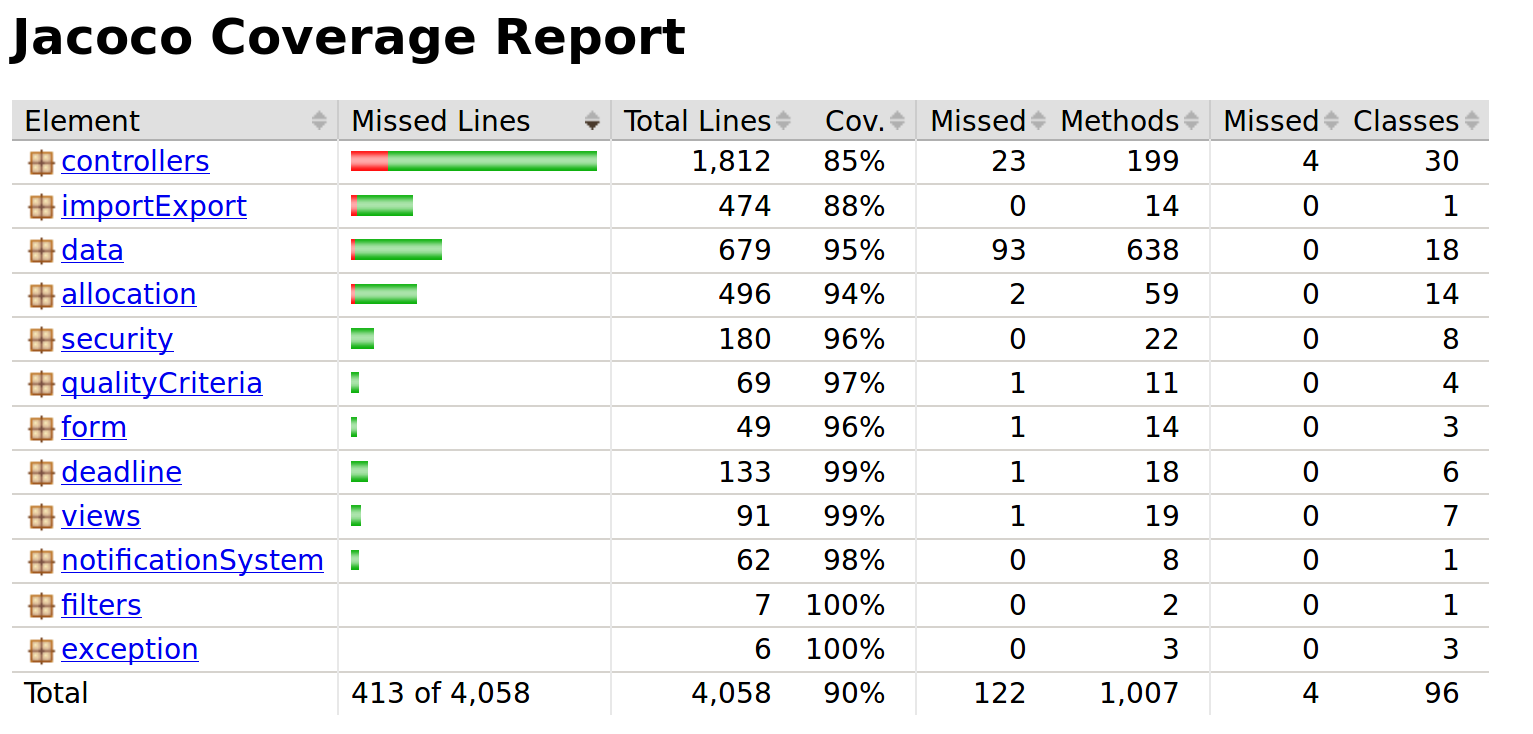
\includegraphics[width=\linewidth]{jacoco.png}

\caption{Die Codezeilen-Überdeckung durch Tests}
\end{figure}


\begin{figure}
	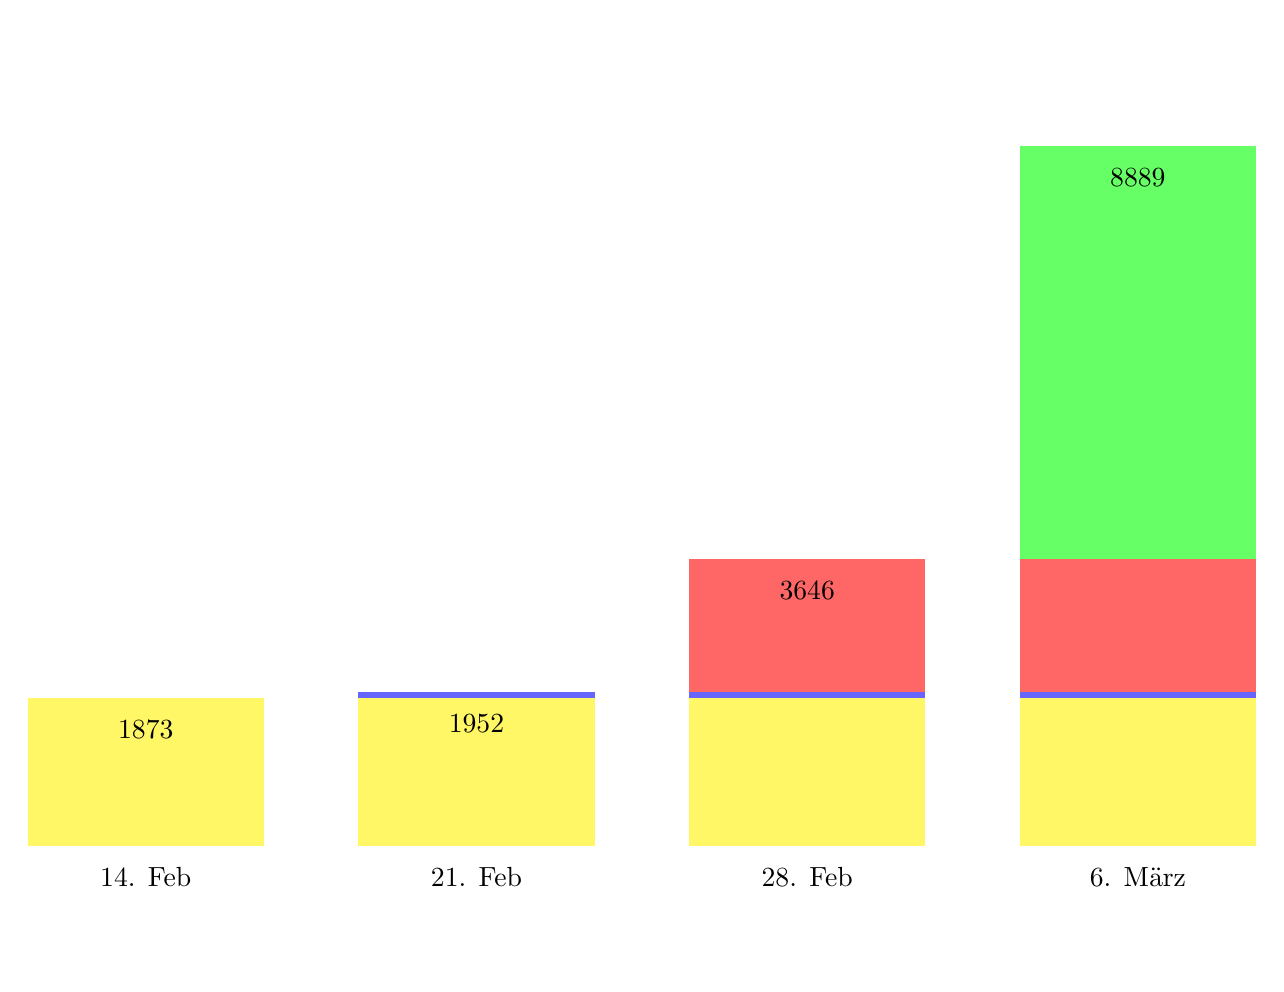
\begin{tikzpicture}[x={(1.4mm,0mm)},y={(0mm,1mm)}]
	\draw[yshift=-4mm] (0,0) node{14. Feb} (30, 0) node{21. Feb} (60, 0) node{28. Feb} (90,0) node{6. März};
	\draw[line width=30mm,green!60] (0,0) plot [ycomb]
	coordinates {(90,88.89)};
	\draw[line width=30mm,red!60] (0,0) plot [ycomb]
	coordinates {(60,36.46) (90,36.46)};
	\draw[line width=30mm,blue!60] (0,0) plot [ycomb]
	coordinates {(30,19.52) (60, 19.52) (90,19.52)};
	\draw[line width=30mm,yellow!60] (0,0) plot [ycomb]
	coordinates {(0,18.73) (30,18.73) (60, 18.73) (90,18.73)};
	\draw[yshift=-4mm](0,18.73) node{1873} (30, 19.52) node{1952} (60, 36.46) node{3646} (90, 88.89) node{8889};
	
	\end{tikzpicture}
	\caption{LOC über die vier Wochen}
\end{figure}

\subsection{Sonarqube}
Zur statischen Codeanalyse haben wir das Werkzeug \enquote{Sonarqube} verwendet. Dadurch sind wir noch einmal auf die im Folgende aufgezählten kleinerer Fehler aufmerksam geworden, wobei durch Sonarqube keine schwerwiegenden Fehlfunktionen aufgedeckt werden konnten. Die Anzahlen beziehen sich auf die Änderung von der ersten Analyse am Ende der Implementierungsphase bis zum Ende der Qualitätssicherung. \enquote{fixed} bedeutet dabei, dass der Fehler behoben wurde, \enquote{false positive}, dass Sonarqube einen Fehler angezeigt hat, den wir nach ausgiebiger Untersuchung als Fehlalarm eingestuft haben und \enquote{removed}, dass diese Regeln aus diversen Gründen nicht auf unser Projekt anwendbar waren. So waren z.B. 158 der entfernten Bugs Aufforderungen einen Logger zu verwenden, wogegen wir uns zu Beginn des Projektes entschieden haben.
\begin{itemize}[noitemsep]
	\item \textbf{Bugs} 
	
	Von Sonarqube per default als Bug klassifizierte Fehler: 0
	\begin{itemize}
		\item 37 fixed
		\item 5 false positive
		\item 163 removed
	\end{itemize}
	\item \textbf{Vulnerabilities}
	 
	Von Sonarqube per default als Sicherheitslücke klassifizierte Fehler: 2
	\begin{itemize}
		\item 3 gefixed
		\item 1 false positive
	\end{itemize}
	\item \textbf{Code Smells} 
	
	Von Sonarqube per default als schlechter Stil klassifizierte Fehler: 168
	\begin{itemize}
		\item 12 gefixed
		\item 32 removed
	\end{itemize}
\end{itemize}

Insgesamt haben wir damit das Sonarqube Standard Quality Gate bestanden.



\end{document}